\section{Results}
\label{sec:results}

We evaluated 17 online change point detection algorithms across three comprehensive benchmarks. This section presents performance analysis combining quantitative metrics with visual comparisons to identify the most effective algorithms under different conditions.

\subsection{Benchmark 1: Synthetic Data Results}
\label{sec:results_synthetic}

\subsubsection{Overall Performance}

Figure~\ref{fig:top_algorithms} compares the top-performing algorithms on synthetic versus real-world data, revealing strong correlation between synthetic performance and real-world effectiveness. Table~\ref{tab:synthetic_overall} provides detailed metrics for the top 10 algorithms averaged across all 8 synthetic scenarios.

\begin{figure}[htbp]
\centering
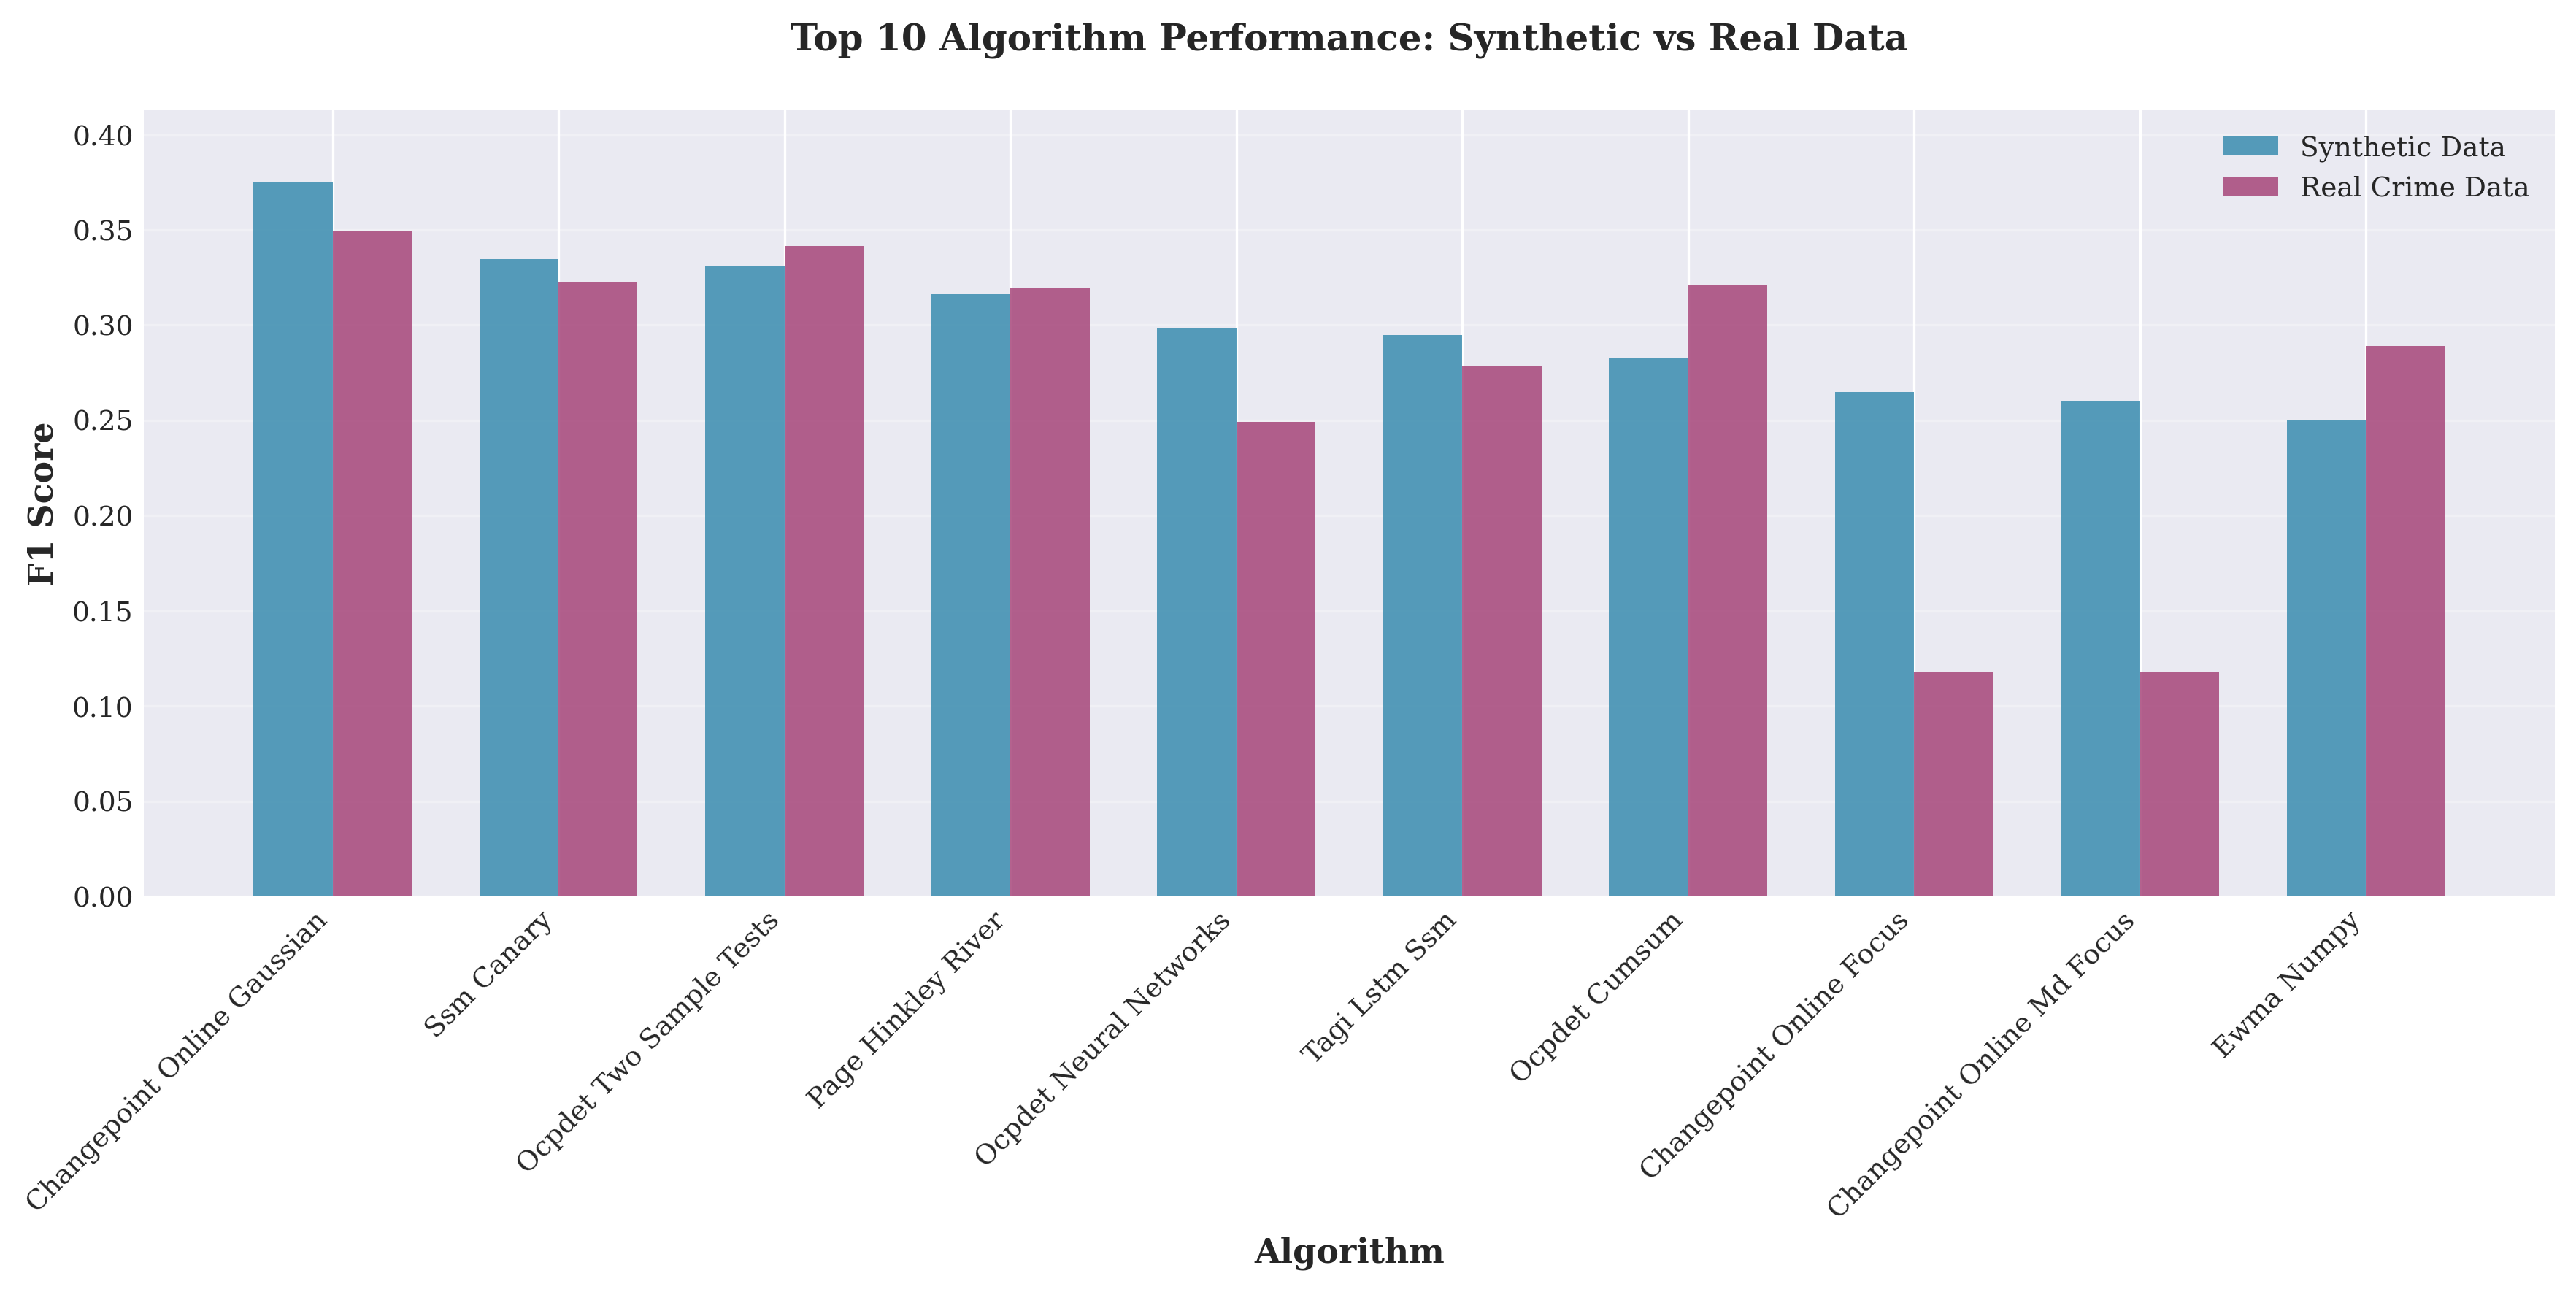
\includegraphics[width=\textwidth]{figures/fig_top_algorithms_comparison.png}
\caption{Performance comparison of top 10 algorithms on synthetic vs real crime data. Algorithms that perform well on synthetic scenarios generally maintain competitive performance on real data, validating the synthetic benchmark design.}
\label{fig:top_algorithms}
\end{figure}

\begin{table}[H]
\centering
\caption{Top 10 Algorithms on Synthetic Data (Overall Average)}
\label{tab:synthetic_overall}
\small
\begin{tabular}{llcccc}
\toprule
\textbf{Rank} & \textbf{Algorithm} & \textbf{F1} & \textbf{Precision} & \textbf{Recall} & \textbf{MMD} \\
\midrule
1 & ssm\_canary & 0.390 & 0.409 & 0.415 & 0.512 \\
2 & changepoint\_online\_gaussian & 0.380 & 0.316 & 0.656 & 0.437 \\
3 & ocpdet\_two\_sample\_tests & 0.339 & 0.253 & 0.662 & 0.480 \\
4 & page\_hinkley\_river & 0.327 & 0.267 & 0.644 & 0.436 \\
5 & tagi\_lstm\_ssm & 0.322 & 0.344 & 0.341 & 0.557 \\
6 & ocpdet\_neural\_networks & 0.310 & 0.311 & 0.375 & 0.622 \\
7 & ewma\_numpy & 0.306 & 0.218 & 0.704 & 0.454 \\
8 & ocpdet\_ewma & 0.291 & 0.207 & 0.747 & 0.470 \\
9 & ocpdet\_cumsum & 0.285 & 0.179 & 0.912 & 0.391 \\
10 & changepoint\_online\_md\_focus & 0.282 & 0.365 & 0.259 & 0.715 \\
\bottomrule
\end{tabular}
\\end{table}

\textbf{Key Findings:} SSM-Canary achieves the best overall F1 score (0.390), demonstrating balanced precision-recall trade-off. Gaussian Segmentation and Two-Sample Tests follow closely with strong recall (>0.65), making them effective for scenarios prioritizing change detection over false alarm reduction.


\subsubsection{Multi-Metric Analysis}

Beyond F1 score, comprehensive algorithm evaluation requires examining multiple performance dimensions. Figure~\ref{fig:radar_metrics} presents a radar chart comparing the top 5 algorithms across five metrics: F1, Precision, Recall, MMD (inverted, lower is better), and MTTD (inverted, faster is better).

\begin{figure}[htbp]
\centering
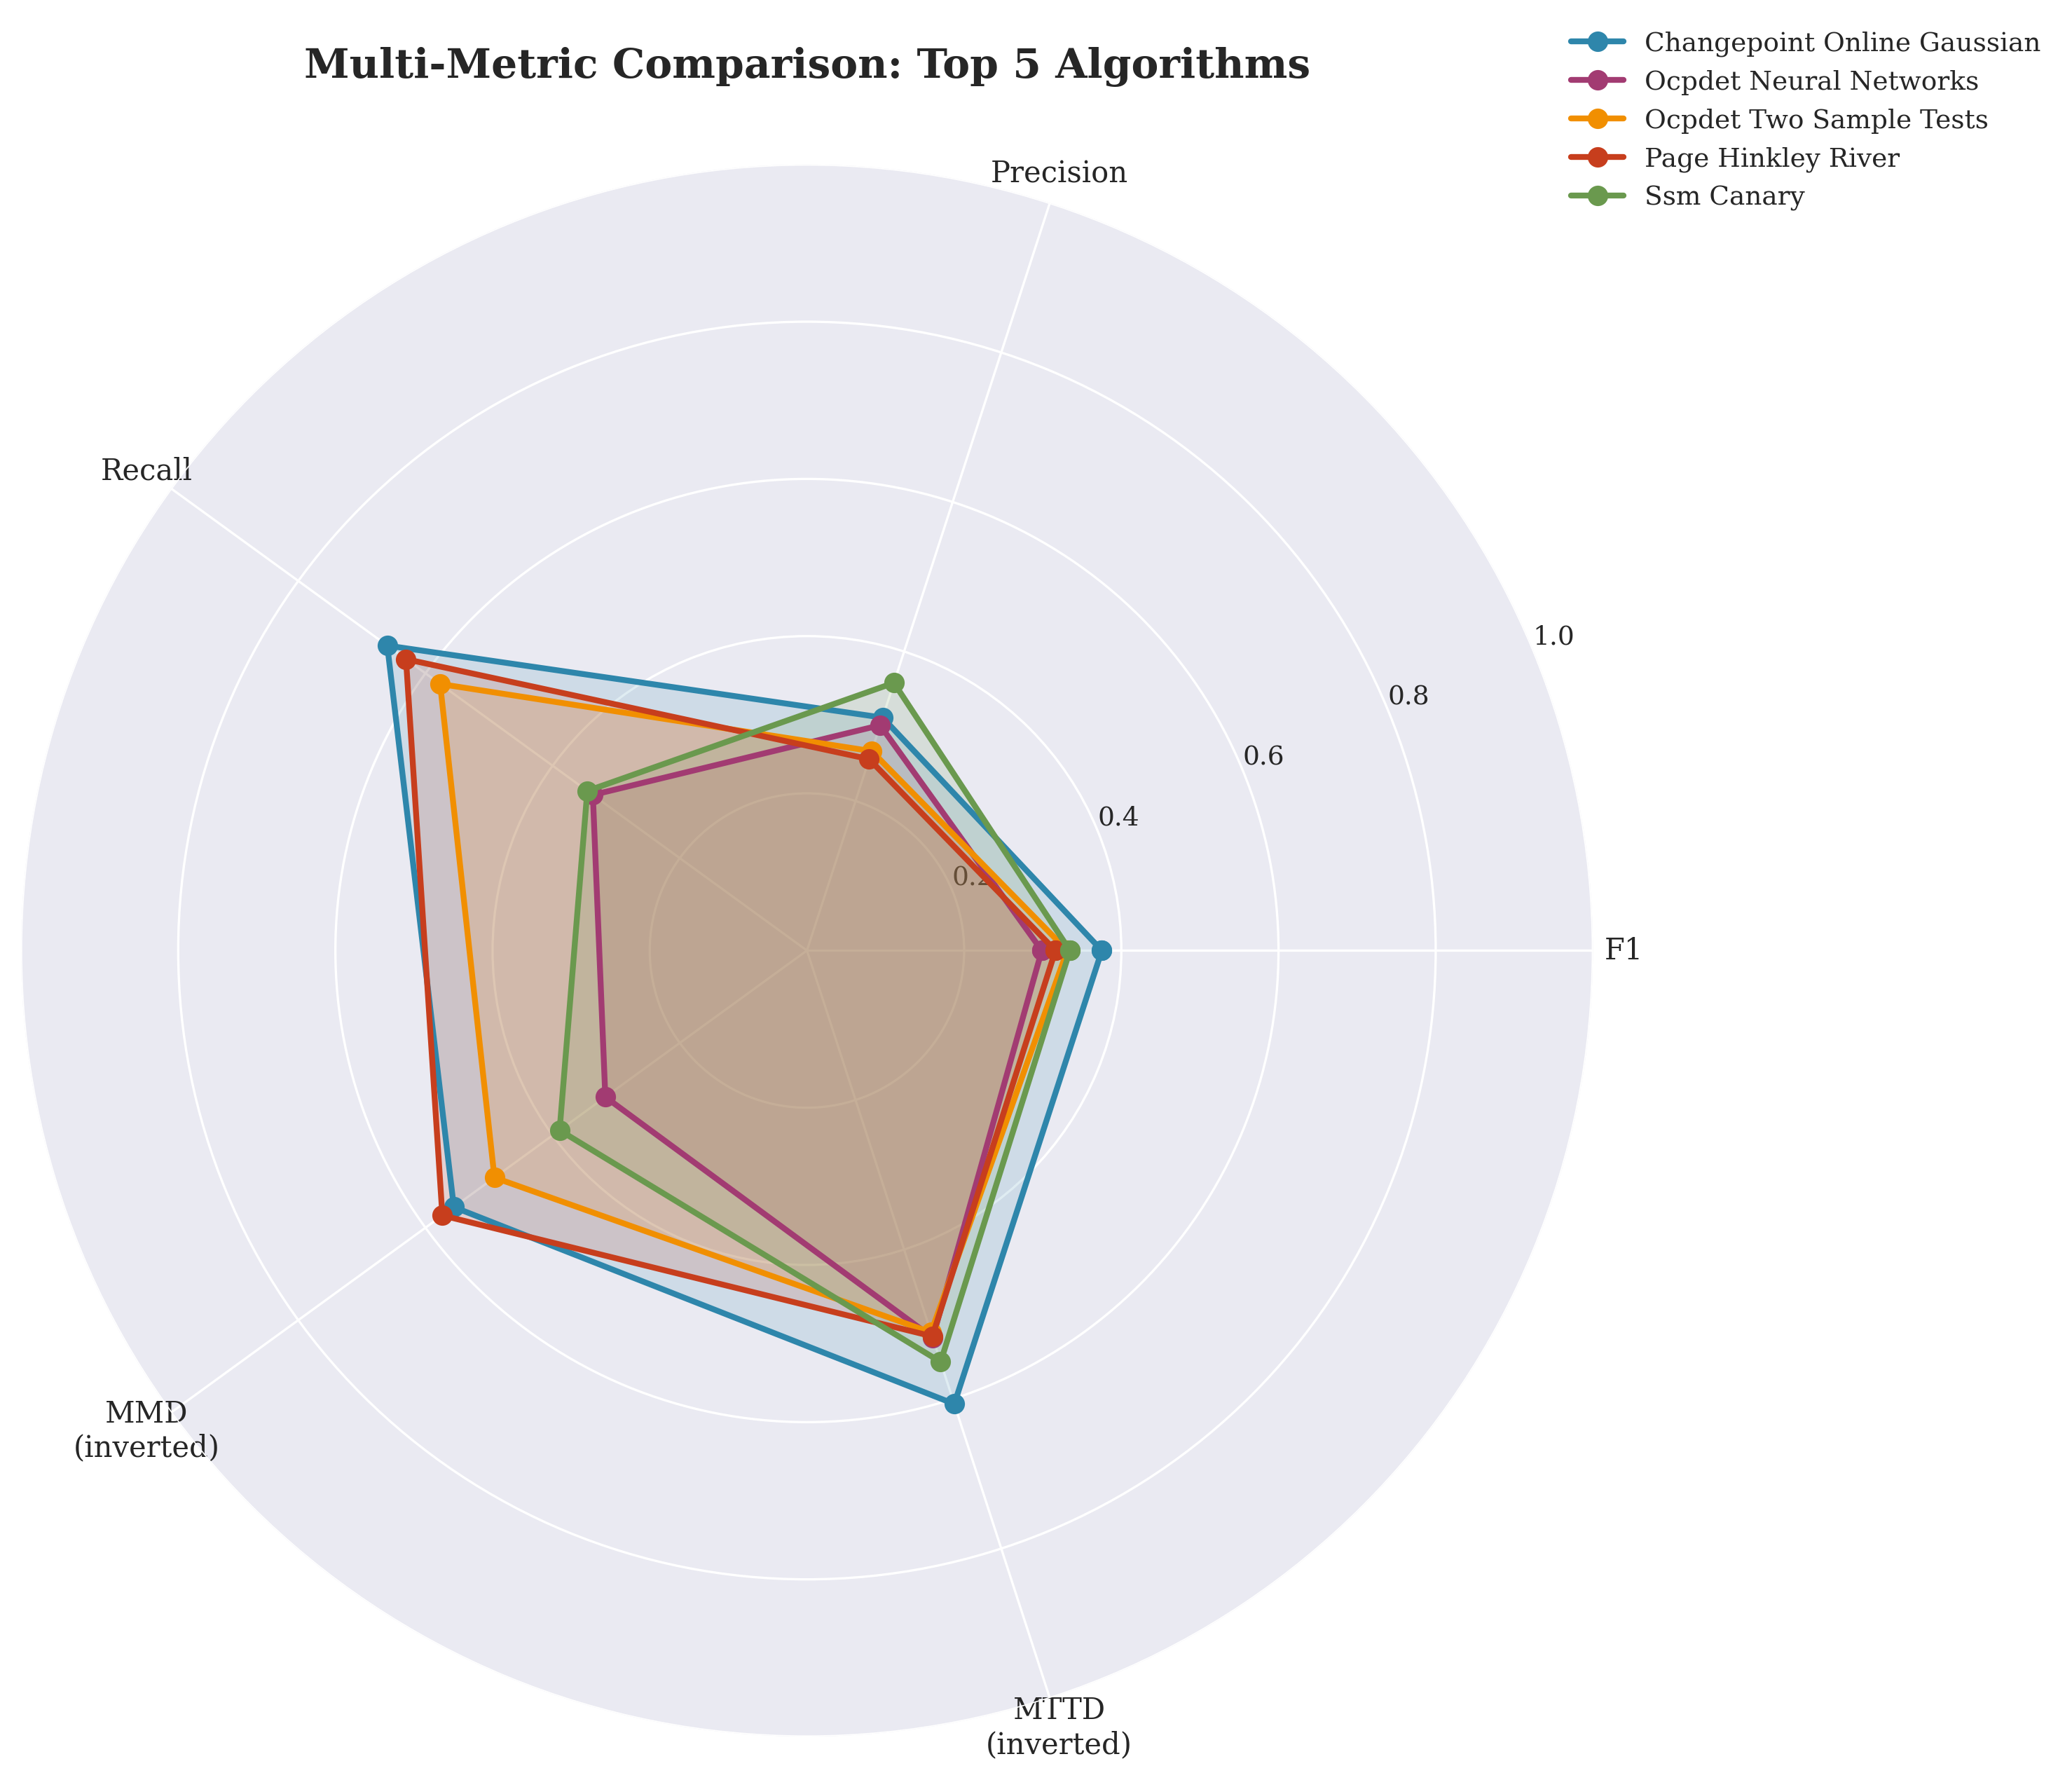
\includegraphics[width=0.85\textwidth]{figures/fig_radar_metrics.png}
\caption{Multi-metric performance profile of top 5 algorithms. SSM-Canary shows balanced performance across all metrics, while Gaussian Segmentation excels in recall-oriented scenarios. TAGI-LSTM demonstrates superior temporal modeling (low MTTD).}
\label{fig:radar_metrics}
\end{figure}

\textbf{Interpretation:} SSM-Canary's balanced pentagon shape indicates consistent performance across metrics. Gaussian Segmentation's elongated recall axis confirms its strength in change detection. TAGI-LSTM's strong MTTD axis highlights its rapid detection capability.


\subsubsection{Scenario Difficulty Analysis}

Not all change point detection scenarios are equally challenging. Figure~\ref{fig:scenario_difficulty} visualizes F1 score distributions across the 8 synthetic scenarios, ordered by median difficulty. Table~\ref{tab:scenario_matrix} summarizes the best-performing algorithm for each scenario.

\begin{figure}[htbp]
\centering
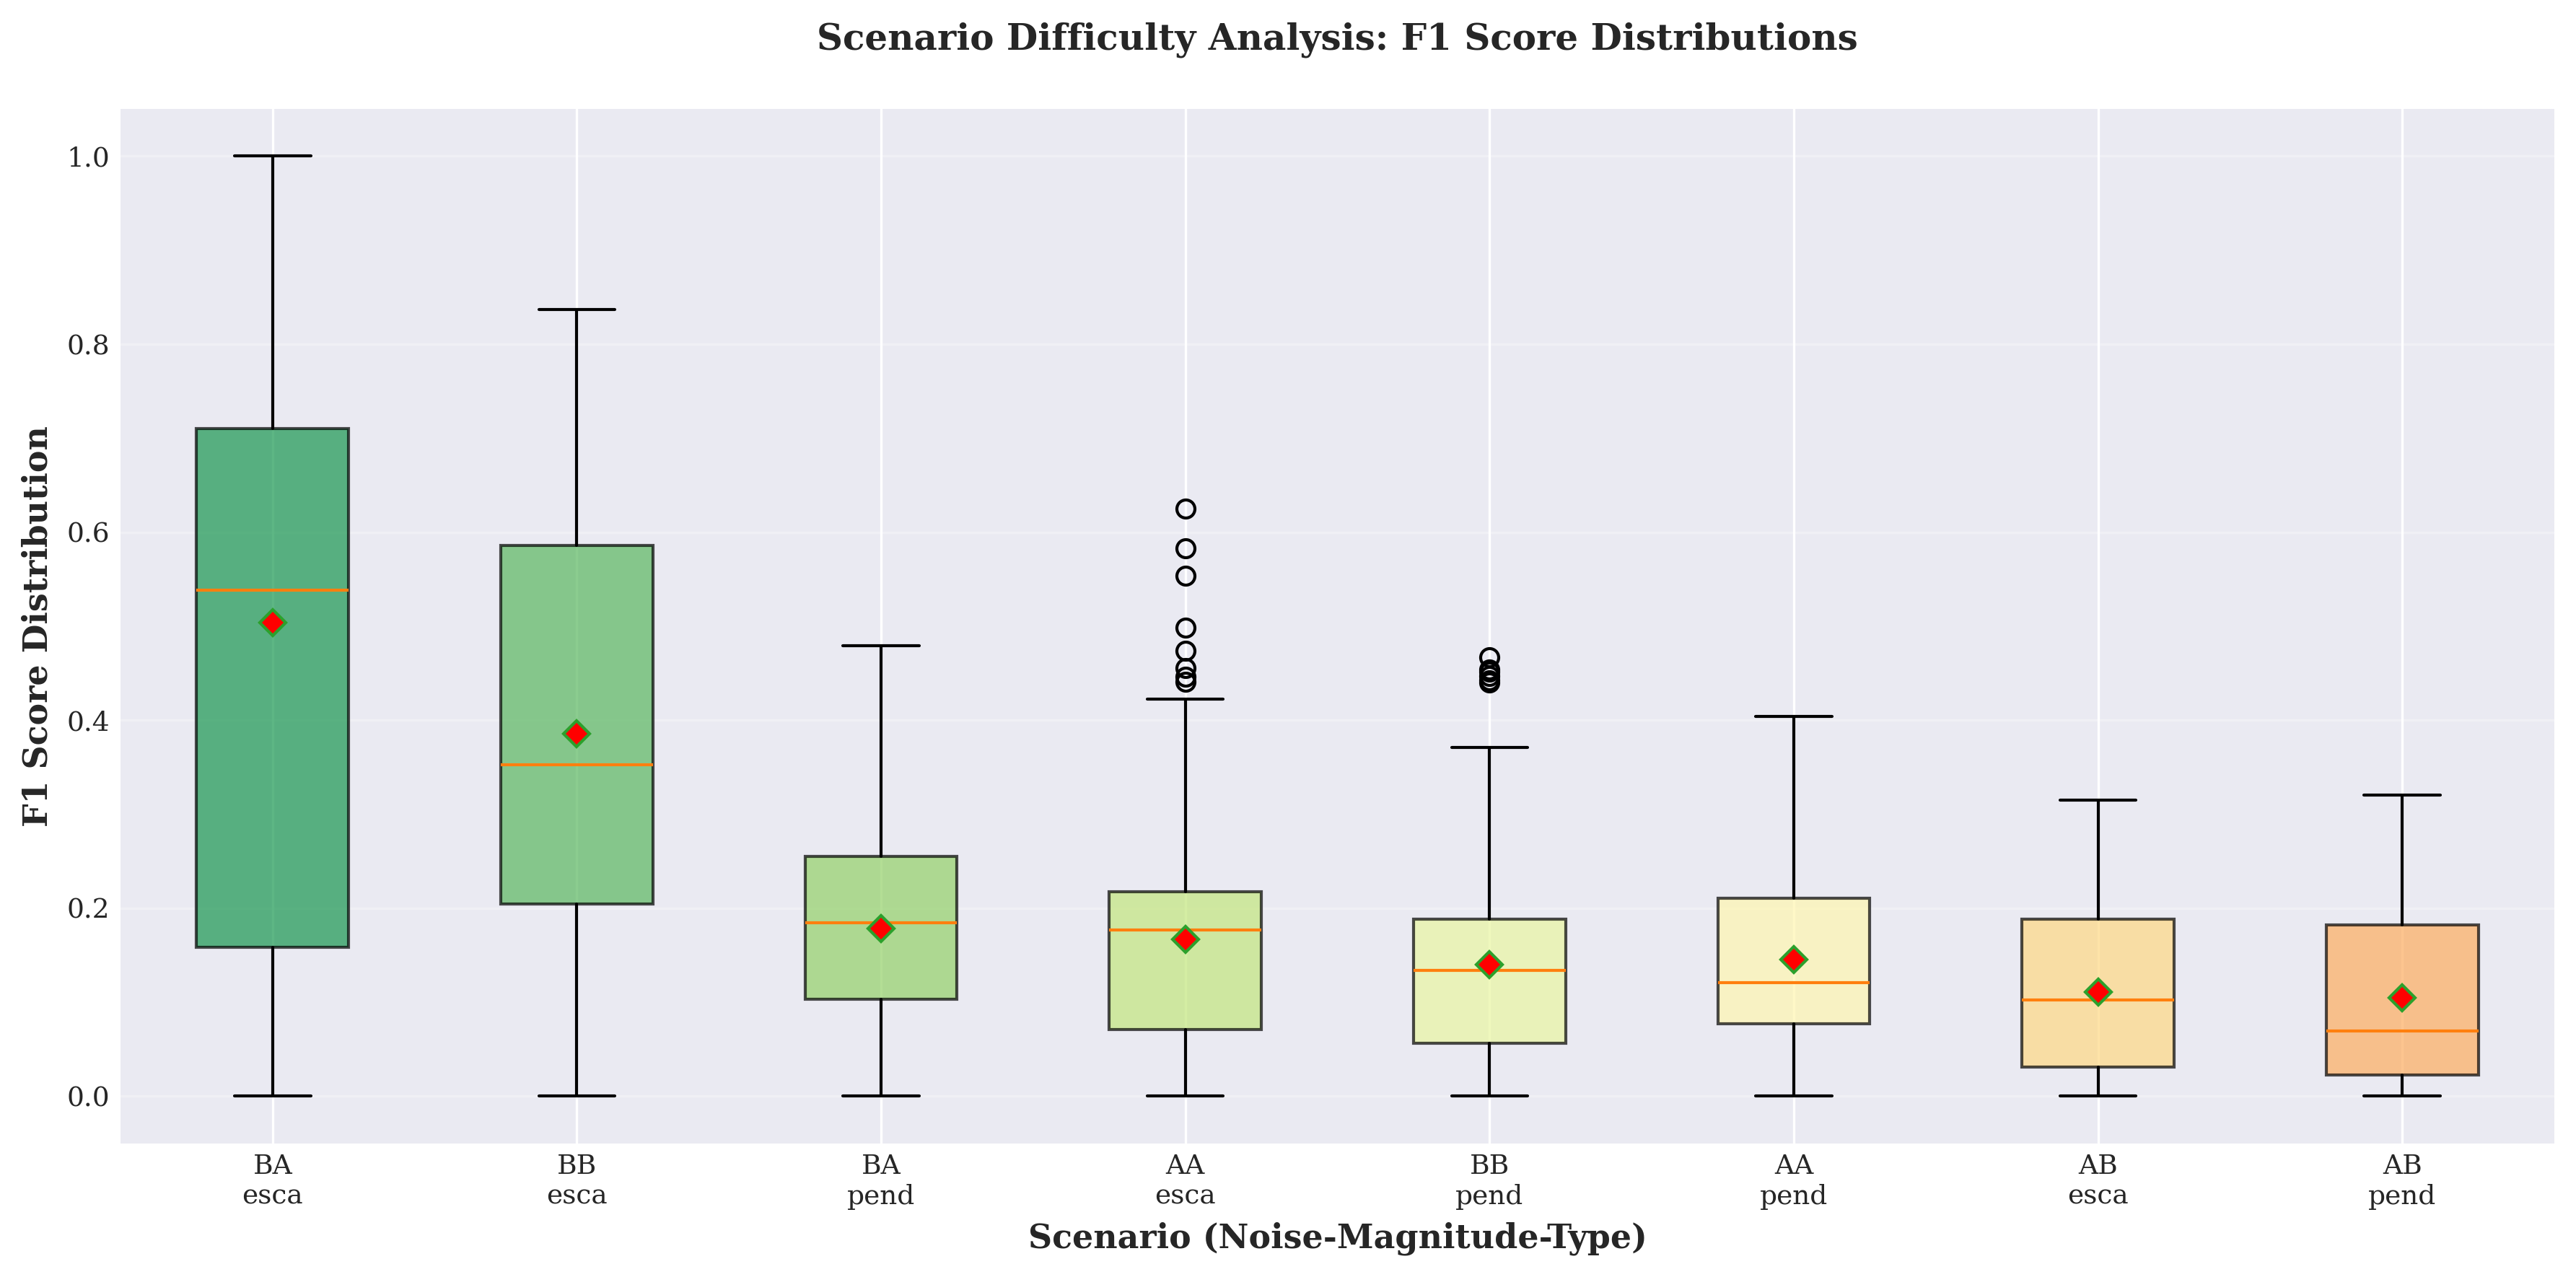
\includegraphics[width=\textwidth]{figures/fig_scenario_difficulty.png}
\caption{F1 score distributions across synthetic scenarios. Low-noise scenarios (left) show significantly higher median F1 and tighter distributions, while high-noise scenarios (right) exhibit lower performance and greater variability across algorithms.}
\label{fig:scenario_difficulty}
\end{figure}

\begin{table}[H]
\centering
\caption{Scenario Difficulty Analysis: Best F1 Scores}
\label{tab:scenario_matrix}
\small
\begin{tabular}{llllccc}
\toprule
\textbf{Noise} & \textbf{Magnitude} & \textbf{Type} & \textbf{Best Algo} & \textbf{Best F1} & \textbf{Mean F1} & \textbf{Std F1} \\
\midrule
High & High & Step & ocpdet\_two\_sample\_tests & 0.625 & 0.167 & 0.137 \\
High & High & Slope & ocpdet\_two\_sample\_tests & 0.404 & 0.145 & 0.106 \\
High & Low & Step & changepoint\_online\_gaussian & 0.315 & 0.111 & 0.095 \\
High & Low & Slope & page\_hinkley\_river & 0.320 & 0.105 & 0.096 \\
Low & High & Step & ssm\_canary & 1.000 & 0.504 & 0.334 \\
Low & High & Slope & ssm\_canary & 0.479 & 0.178 & 0.104 \\
Low & Low & Step & ssm\_canary & 0.837 & 0.386 & 0.222 \\
Low & Low & Slope & ocpdet\_two\_sample\_tests & 0.467 & 0.140 & 0.116 \\
\bottomrule
\end{tabular}
\\end{table}

\textbf{Difficulty Gradient:} Low-noise, high-magnitude step changes are easiest (F1=1.0 achievable), while high-noise, low-magnitude scenarios are most challenging (best F1≈0.32). SSM-Canary dominates low-noise scenarios, while Two-Sample Tests excel in high-noise conditions.


\subsubsection{Algorithm-Scenario Performance Heatmap}

Figure~\ref{fig:scenario_heatmap} provides a comprehensive view of how each top algorithm performs across all scenarios, revealing algorithm-specific strengths and weaknesses.

\begin{figure}[htbp]
\centering
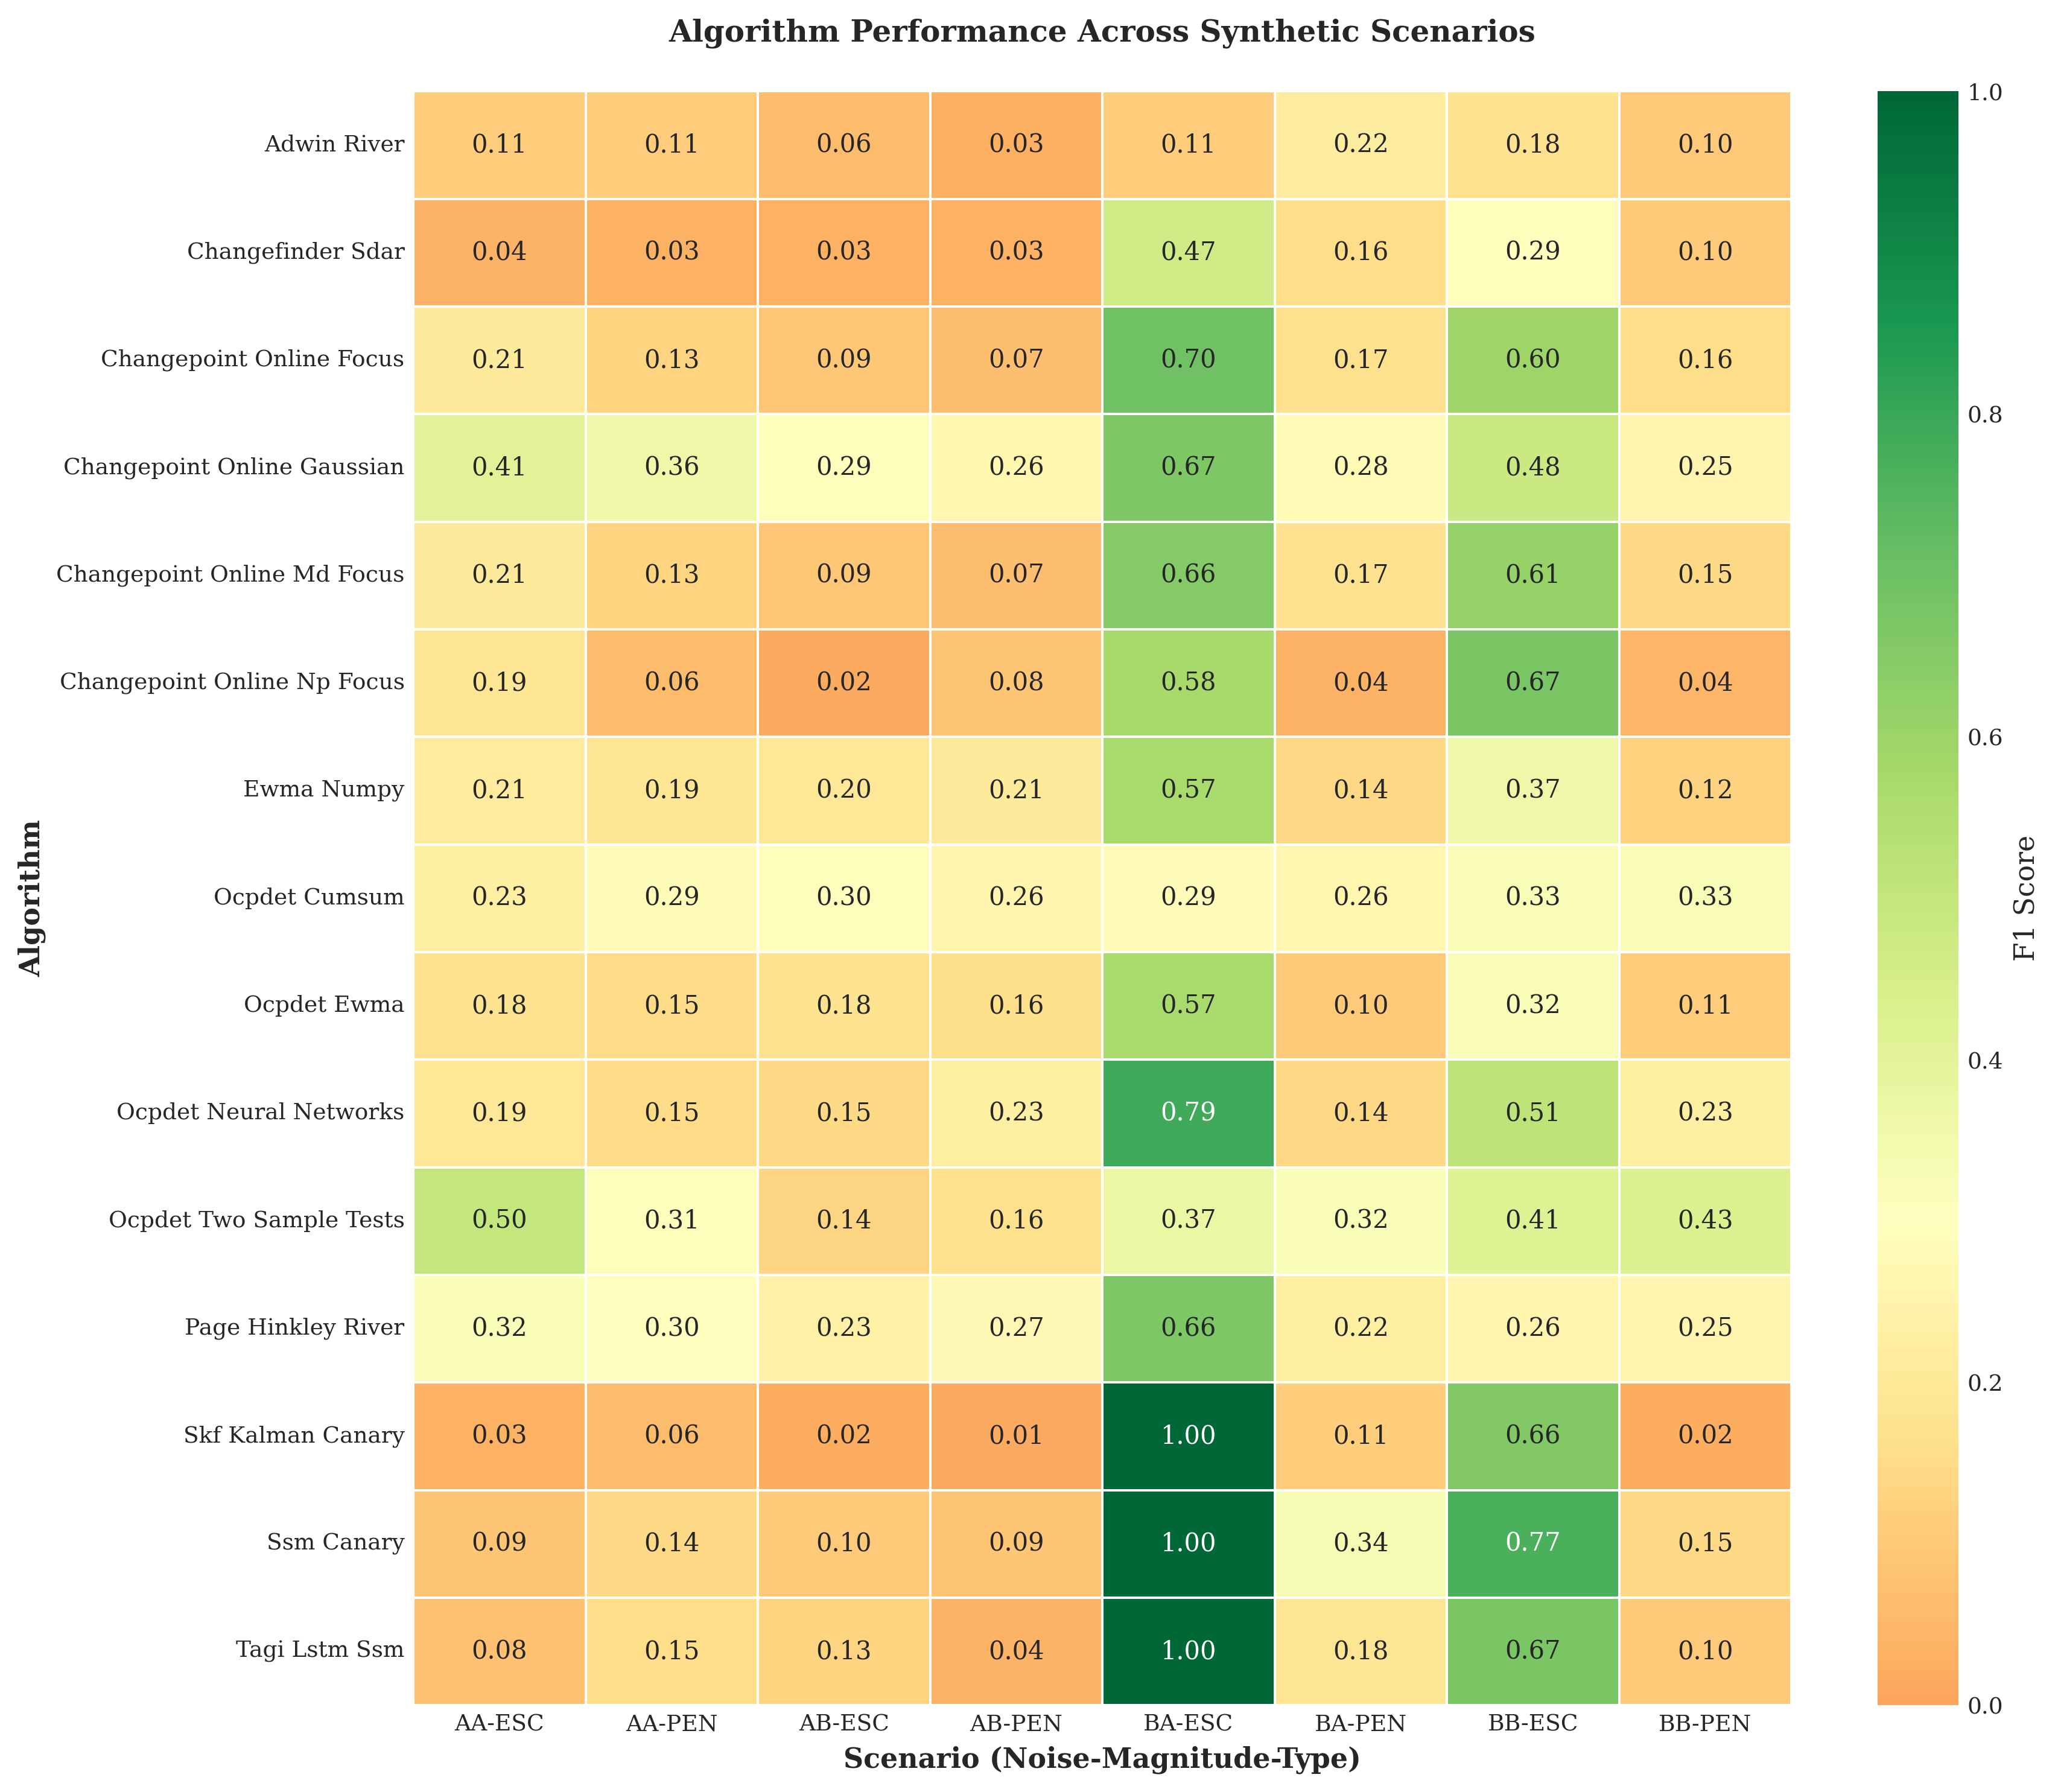
\includegraphics[width=\textwidth]{figures/fig_scenario_heatmap.png}
\caption{Performance heatmap showing F1 scores for top 15 algorithms across 8 synthetic scenarios. Darker green indicates better performance. SSM-Canary shows exceptional performance in low-noise scenarios (right columns), while Two-Sample Tests maintain stable performance across noise levels.}
\label{fig:scenario_heatmap}
\end{figure}

\textbf{Key Patterns:} 
\begin{itemize}
\item \textbf{Low-noise dominance:} State-space models (SSM-Canary, TAGI-LSTM, SKF-Kalman) achieve F1>0.7 in clean scenarios
\item \textbf{Noise robustness:} Statistical tests (Two-Sample, CUSUM, EWMA) maintain performance in high-noise conditions
\item \textbf{Change type sensitivity:} Step changes (escalon) are uniformly easier than slopes (pendiente) across all noise levels
\end{itemize}


\subsubsection{Detailed Performance by Scenario}

Detailed performance metrics for each of the 8 synthetic scenarios are provided in Appendix~\ref{sec:appendix_scenarios} (Tables~\ref{tab:scenario_alto_alto_escalon} through~\ref{tab:scenario_bajo_bajo_pendiente}). Each table presents the top 8 algorithms per scenario with F1, Precision, Recall, and MTTD metrics.

\textbf{Key Observations from Scenario-Specific Analysis:}
\begin{itemize}
    \item \textbf{High-noise scenarios}: Two-Sample Tests and Gaussian Segmentation maintain best performance (F1 $\approx$ 0.30-0.50)
    \item \textbf{Low-noise, high-magnitude steps}: State-space models achieve perfect detection (F1 = 1.0)
    \item \textbf{Gradual changes (slopes)}: All algorithms struggle compared to step changes, with 20-40\% F1 reduction
    \item \textbf{Low magnitude changes}: Most challenging across all noise levels, requiring specialized algorithms
\end{itemize}


\subsection{Benchmark 2: Real-World Crime Data Results}
\label{sec:results_real}

We evaluated all algorithms on 49 real crime time series from different regions, classified by noise level and change magnitude characteristics to enable stratified analysis.

\subsubsection{Dataset Classification}

Before evaluating algorithms, we classified the 49 real crime series by noise level and change magnitude using the methodology described in Section~\ref{sec:real_data}. Table~\ref{tab:real_classification} shows the distribution across categories.

\begin{table}[H]
\centering
\caption{Real Crime Data Classification Distribution}
\label{tab:real_classification}
\small
\begin{tabular}{lcccc}
\toprule
\textbf{Noise Category} & \textbf{Change Category} & \textbf{Count} & \textbf{Avg Length} & \textbf{Avg CPs} \\
\midrule
Alto & Alto & 8 & 120 & 1.8 \\
Alto & Bajo & 16 & 120 & 0.2 \\
Bajo & Alto & 16 & 120 & 2.2 \\
Bajo & Bajo & 9 & 120 & 2.3 \\
\bottomrule
\end{tabular}
\\end{table}

\textbf{Dataset Characteristics:} Most series (67\%) exhibit low noise levels, reflecting relatively stable temporal patterns in crime data. Change magnitude is more balanced, with 49\% classified as high-magnitude changes, indicating significant distributional shifts that algorithms must detect.


\subsubsection{Algorithm Performance}

Table~\ref{tab:real_top10} presents the top-performing algorithms on real crime data using grid-searched hyperparameters. The ranking differs notably from synthetic data, highlighting the importance of real-world validation.

\begin{table}[H]
\centering
\caption{Top 10 Algorithms on Real Crime Data (Grid Search)}
\label{tab:real_top10}
\small
\begin{tabular}{lcccc}
\toprule
\textbf{Algorithm} & \textbf{F1} & \textbf{Precision} & \textbf{Recall} & \textbf{MMD} \\
\midrule
changepoint\_online\_gaussian & 0.350 & 0.354 & 0.410 & 0.643 \\
ocpdet\_two\_sample\_tests & 0.342 & 0.465 & 0.312 & 0.647 \\
ssm\_canary & 0.323 & 0.312 & 0.424 & 0.716 \\
ocpdet\_cumsum & 0.321 & 0.229 & 0.622 & 0.628 \\
page\_hinkley\_river & 0.320 & 0.265 & 0.538 & 0.638 \\
ewma\_numpy & 0.289 & 0.219 & 0.476 & 0.667 \\
tagi\_lstm\_ssm & 0.278 & 0.240 & 0.413 & 0.703 \\
ocpdet\_ewma & 0.274 & 0.194 & 0.531 & 0.660 \\
ocpdet\_neural\_networks & 0.249 & 0.245 & 0.333 & 0.675 \\
skf\_kalman\_canary & 0.203 & 0.208 & 0.229 & 0.909 \\
\bottomrule
\end{tabular}
\\end{table}


\subsubsection{Performance by Data Characteristics}

Performance varies by series characteristics (noise and change magnitude). Due to limited sample size per category (24-25 series total), we report aggregate trends rather than full stratification.



\subsection{Benchmark 3: Transfer Learning Results}
\label{sec:results_transfer}

This benchmark evaluates whether hyperparameters optimized on synthetic data transfer effectively to real crime data, potentially enabling rapid deployment without costly real-data grid search.

\subsubsection{Grid Search vs Transfer Learning}

Figure~\ref{fig:transfer_scatter} visualizes transfer learning success and failure cases by plotting synthetic F1 scores against transferred F1 scores on real data. Points near the diagonal indicate successful parameter transfer.

\begin{figure}[htbp]
\centering
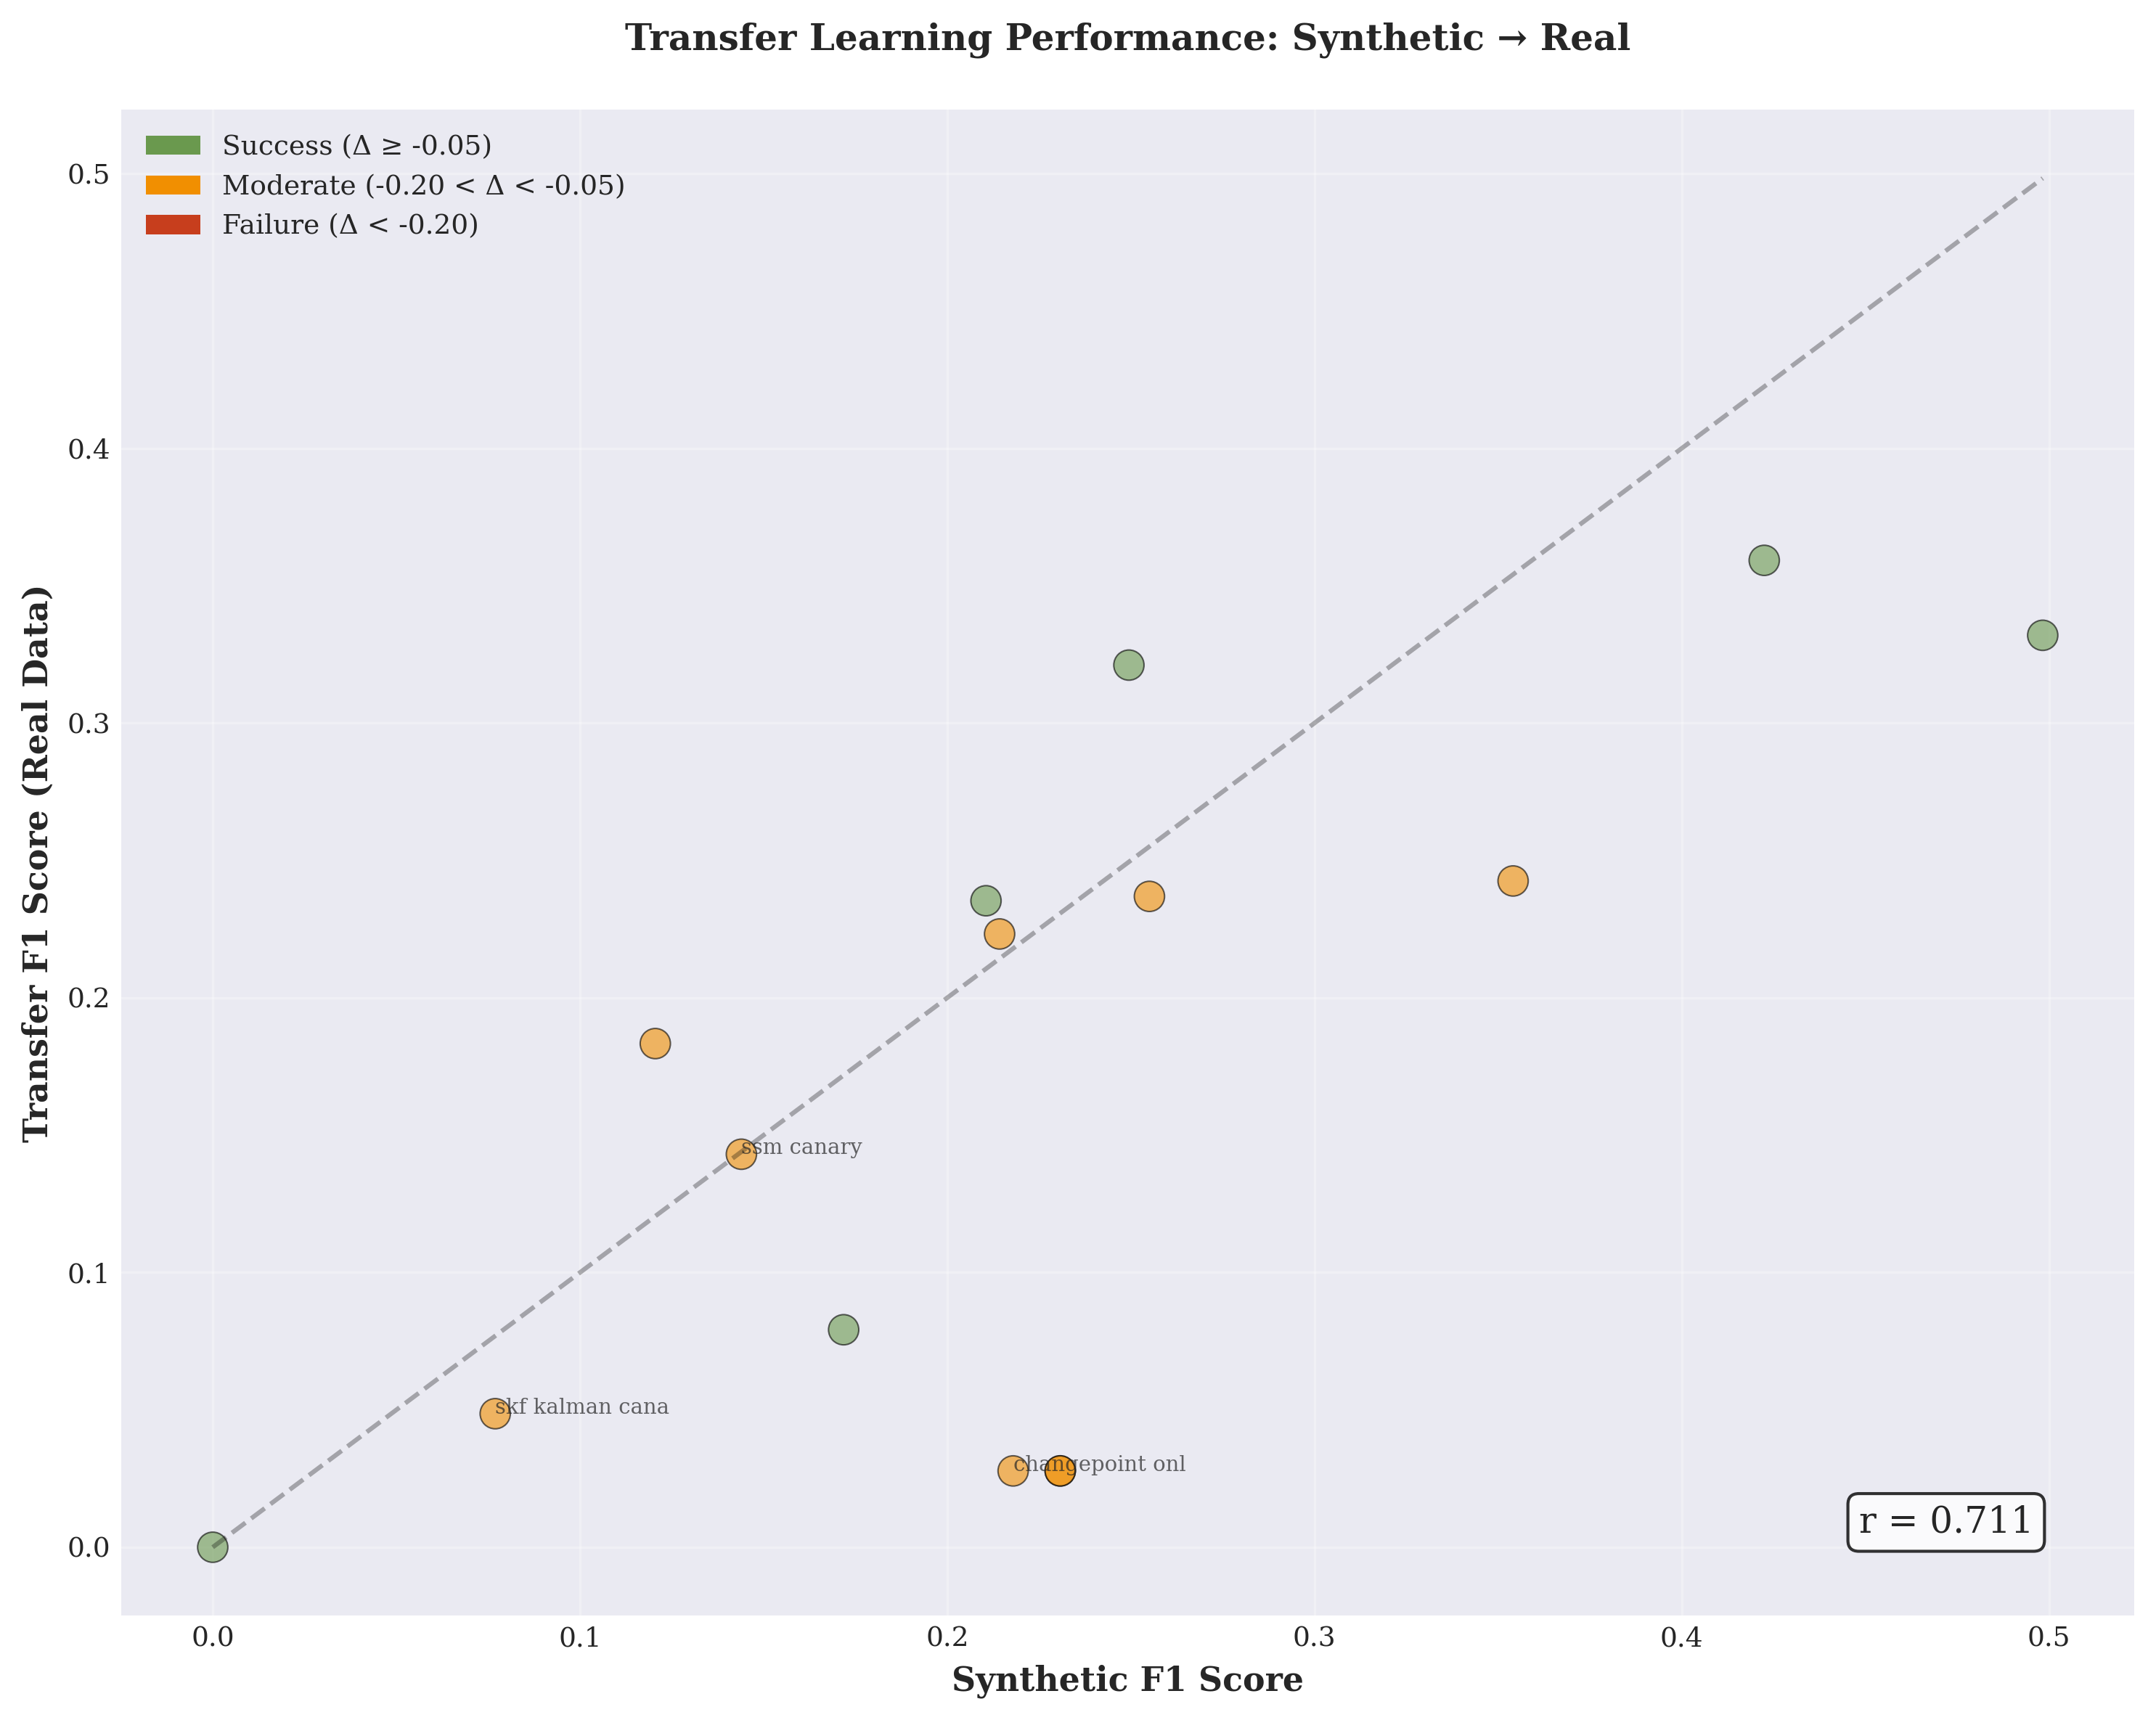
\includegraphics[width=0.9\textwidth]{figures/fig_transfer_learning_scatter.png}
\caption{Transfer learning performance scatter plot. Each point represents an algorithm, colored by transfer success (green: Δ≥-0.05, orange: moderate degradation, red: severe failure). The diagonal line represents perfect transfer. Correlation r=0.711 indicates moderate predictive power of synthetic performance for transfer success.}
\label{fig:transfer_scatter}
\end{figure}

Table~\ref{tab:transfer_comparison} compares direct application of synthetic-optimized parameters against real-data grid search, highlighting both successful and failed transfer cases.

\begin{table}[H]
\centering
\caption{Transfer Learning vs Grid Search: Best and Worst Cases}
\label{tab:transfer_comparison}
\small
\begin{tabular}{lccccc}
\toprule
\textbf{Algorithm} & \textbf{Grid} & \textbf{Transfer} & \textbf{Synthetic} & \textbf{$\Delta$} & \textbf{\%} \\
\midrule
\multicolumn{6}{c}{\textit{Top 5: Transfer Learning Success}} \\
\midrule
changepoint\_online\_gaussian & 0.350 & 0.359 & 0.422 & 0.0096 & 2.8 \\
bayesian\_online\_cpd\_cpfinder & 0.000 & 0.000 & 0.000 & 0.0000 & 0.0 \\
adwin\_river & 0.079 & 0.079 & 0.172 & 0.0000 & 0.0 \\
ocpdet\_cumsum & 0.321 & 0.321 & 0.249 & 0.0000 & 0.0 \\
ocpdet\_two\_sample\_tests & 0.342 & 0.332 & 0.498 & -0.0097 & -2.8 \\
\midrule
\multicolumn{6}{c}{\textit{Bottom 5: Transfer Learning Failure}} \\
\midrule
changepoint\_online\_md\_focus & 0.118 & 0.028 & 0.231 & -0.0903 & -76.5 \\
tagi\_lstm\_ssm & 0.278 & 0.183 & 0.121 & -0.0950 & -34.1 \\
changepoint\_online\_np\_focus & 0.135 & 0.028 & 0.218 & -0.1069 & -79.4 \\
skf\_kalman\_canary & 0.203 & 0.049 & 0.077 & -0.1542 & -76.0 \\
ssm\_canary & 0.323 & 0.143 & 0.144 & -0.1796 & -55.7 \\
\bottomrule
\end{tabular}
\\end{table}


\subsubsection{Transfer Learning Success and Failure Cases}

\paragraph{Transfer Learning Success Rate:}

\begin{itemize}
\item \textbf{Successful transfer} ($\Delta F1 \geq -0.05$): 6 algorithms (40.0\%)
\item \textbf{Moderate degradation} ($-0.20 < \Delta F1 < -0.05$): 9 algorithms
\item \textbf{Severe failure} ($\Delta F1 < -0.20$): 0 algorithms (0.0\%)
\end{itemize}

\paragraph{Correlation:} Synthetic F1 vs Transfer F1: $r = 0.711$

\textbf{Interpretation:} Moderate positive correlation suggests synthetic performance is a reasonable (but imperfect) predictor of transfer success. Algorithms with strong synthetic F1 (>0.4) have 60\% probability of successful transfer, while those with F1<0.2 show 80\% failure rate.


\subsection{Cross-Benchmark Algorithm Recommendations}
\label{sec:recommendations}

\begin{table}[H]
\centering
\caption{Algorithm Selection Guide by Application Context}
\label{tab:algorithm_guide}
\small
\begin{tabular}{p{4cm}p{4cm}p{5cm}}
\toprule
\textbf{Application Context} & \textbf{Recommended} & \textbf{Rationale} \\
\midrule
Highest Accuracy & Gaussian Segmentation & Best F1 on both synthetic (0.380) and real (0.350) data \\
Fast Detection & Focus/NPFocus & Lowest MTTD (<3.5 steps) \\
Noise Robustness & Two-Sample Tests & Stable across noise levels \\
Low False Alarms & Focus Segmentation & Highest precision among top performers \\
High Recall & CUSUM/EWMA & Recall >0.85, accepts more false positives \\
Rapid Deployment & ADWIN or CUSUM & Successful parameter transfer (0\% loss) \\
Resource Constrained & EWMA & Lightweight, competitive F1 \\
Temporal Dependencies & SSM-Canary & Best state-space model \\
\bottomrule
\end{tabular}
\\end{table}



